%%
\documentclass{aiaa-tc}% insert '[draft]' option to show overfull boxes
% \documentclass{article}% insert '[draft]' option to show overfull boxes
%%

% list packages between braces
\usepackage{graphicx}
\usepackage{varioref}%  smart page, figure, table, and equation referencing
\usepackage{wrapfig}%   wrap figures/tables in text (i.e., Di Vinci style)
\usepackage{threeparttable}% tables with footnotes
\usepackage{dcolumn}%   decimal-aligned tabular math columns
\newcolumntype{d}{D{.}{.}{-1}}
\usepackage{nomencl}%   nomenclature generation via makeindex
\makeglossary
\usepackage{subfigure}% subcaptions for subfigures
\usepackage{subfigmat}% matrices of similar subfigures, aka small mulitples
\usepackage{fancyvrb}%  extended verbatim environments
\fvset{fontsize=\footnotesize,xleftmargin=2em}
\usepackage{lettrine}%  dropped capital letter at beginning of paragraph
%\usepackage[dvips]{dropping}% alternative dropped capital package
%\usepackage[colorlinks]{hyperref}%  hyperlinks [must be loaded after dropping]
\usepackage{amsmath}

%% Daoru added the following package
\usepackage{multirow}
%%

\begin{document}

\title{CSCI545 Robotics Final Project Report\\
	Robotic Motion Planning}

 \author
{		May Ang%
		\hspace{3pt},
		Thomas Collins%
		\hspace{3pt},
		Justin Garten%
		\hspace{3pt},
		and Michael Joyce%
		\\
		\normalsize\itshape
		University of Southern California, Los Angeles, CA, 90007, USA\\
}
\maketitle

\section{Introduction}
\label{Introduction}

\subsection{Background}

Robots are no longer confined behind striped yellow lines
with flashing lights to keep soft humans away from the moving
parts. They operate in busy hospital hallways, kitchens, and homes
with pets, children, and clutter in a constant state of motion. As
such, the ability to evaluate and interact with those dynamic environments is
increasingly essential for successful operation. \\ \\
There are a number of possible approaches to this, many of which are
strongly influenced by the risks of the environment, nature of the
task, and the type of information to which the robot has
access. If uncertain, should it simply stop and wait for instructions?
Should it push through, trusting others to get out of its way? An
industrial bot capable of ripping through a wall may need to consider very different issues than a robotic vacuum which will at most scuff a
floorboard.
\subsection{Problem Description}

Issues relating to navigation and motion planning run up and down the entire
robotic stack. For the purposes of this project, we chose to consider the high-level planning 
aspects of following a moving goal (tracking a target) in a dynamic environment with a robot whose motion was significantly noisy.
Our primary approach was to explore, extend, and
evaluate three broad categories of methods for this task: Potential Fields, Markov Decision Processes (MDPs), and
reinforcement learning.

\subsection{Robocode Environment}

As the environment for our experiments, we chose to work with a small
framework called Robocode \\(http://robocode.sourceforge.net/). This system is designed for small-scale
simulated robotic tank battles. Users of the system are able to write
the central processing loops for the robotic tanks which have access to
standard sensors, weapons, and motion controls. \\ \\
Several features in particular appealed to us. Its semi-continuous underlying state
representation (locations as doubles) gave us flexibility in
terms of laying a grid over the environment rather than existing in a
pre-defined grid. Critically, this made it far easier to experiment
across methods which required discretization (MDPs and Q-learning) and
those which did not (potential fields). \\ \\
The motion controls proved to be similarly flexible, lending
themselves to discretization when necessary, while leaving access to
the low-level controls where appropriate. \\ \\
The sensors offered a range of options, providing a flexible base
model which was easily extended to account for the particular
structure of individual
experiments. This was abstracted in the Robocode context with the
concept of radar. Basically, each bot had a narrow-band sensor which could be rotated 360 degrees to provide a sweep of the environment and in internal sensor to keep track of its (x, y) position on the battlefield at all times. \\ \\
Finally, the visualization provided by the Robocode framework was an appealing fringe benefit, providing
rapid feedback on experiments and allowing us to more easily evaluate
and iterate. \\ \\
One of the first steps in this project was to evaluate the possible
environments to work in. As our aim was to focus in on the planning and navigation algorithms,
we wanted to work in a context which allowed us to abstract and
encapsulate as many
surrounding issues as possible. After a certain amount of exploration, we did
in-depth evaluations of three options: ROS, a simple grid world, and
Robocode. \\ \\
The primary concern we had about using ROS was the potential for a lengthy setup time.
As none of us had extensive prior experience, our
initial efforts suggested that we might end up spending a good portion
of the project just learning the tools. While this is an environment that all
of us were interested in, even in the best case it would not have left
us a great deal of time to explore the planning and navigation
algorithms we were primarily interested in. \\ \\
The primary concern we had about using a custom grid world was the risk of getting bogged down
in implementation details and being unable to take advantage of any
existing features, particularly in terms of visualization. \\ \\
We settled on the Robocode environment as a good compromise for our
needs. It proved to be a solid choice as it provided us with the
ability to add in features as required while working in a simple
space when needed, not much more complicated than a basic grid world.


\subsection{Report Outline}
In the following three sections, we discuss our efforts to explore
this task using Potential Fields, Markov Decision Processes (MDPs) and
reinforcement learning, specifically Q-learning.

\section{Potential Fields}
\label{Potential Fields}

\subsection{Setup}
The implementation of Potential Fields in Robocode went through a number of steps before coming to a satisfying conclusion. The implementation relies on a few assumptions that Robocode makes possible. First, Robocode always allows the robot get its exact $x$ and $y$ coordinates via \verb|getX()| and \verb|getY()| respectively. The heading of the robot can be gathered from a call to \verb|getHeading()|. The potential field implementations focus on manipulating the heading of the robot and the speed settings to get effective navigation and obstacle avoidance. Potential fields didn't require any special setup like the other methods tested, so jumping into the development was mostly painless.

% Experiments
\subsection{Experiments}
The first goal of potential field implementation was getting a simple proof of concept working in Robocode. The environment was unfamiliar, but fairly simple, so this didn't pose too great a problem. The initial tests were simple single agent environments with a stationary goal. To encode the notion of a ``goal'' in Robocode a stationary bot was used. To calculate the angle of rotation needed to point towards the goal, the robot coordinates and goal coordinates were subtracted and passed to the arctangent variant \verb|Math.atan2()|. This could be used to modify the current heading value, and thus turn the robot towards the goal. \\ \\
While the initial tests worked, the performance was less than stunning. The simple motion model in Robocode was used as opposed to the advanced, which meant that all the robot actions blocked. For this simple example it didn't pose much of a problem, but it made scaling the speed as the bot approached the goal less than ideal. It did cause problems in later tests and would eventually be changed. \\ \\
The next reasonable step seemed to be to use a moving goal since a stationary goal wasn't especially interesting to watch. Again, as with all the tests, a simple robot was used to implement the goal. It was coded to follow a simple pattern around the environment as quickly as possible. The test robot would rotate in a circle until it located the goal. Once the goal was found, it would do its best to continue heading towards the goal.  \\ \\
It was this test that made it evident that the simple motion model wasn't sufficient. While tasks like sweeping the radar can be performed in the simple model, they eat up ticks that the robot could spend doing something else. The bot would end up rotating the radar for one tick, then turning with another tick, and then moving forward with yet another tick. 
\begin{figure}[htb]
\centering
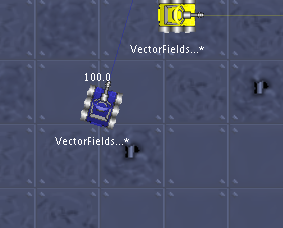
\includegraphics[width=0.5\textwidth]{images/SimpleRadarFailure}
\caption{Notice that the blue robot has lost track of the goal and is tracking an older position.}
\end{figure} \\
In an effort to save ticks and make the motion of the robot smoother, the radar was locked facing forward so the bot would always scan the direction it faced. However, the bot would sometimes lose track of the goal if it passed too close or made sudden direction changes. In addition, because the actions in the simple motion model block, the speed had to be set to the lowest possible setting. If it wasn't, the robot would attempt to move forward some number of units in the environment before doing another radar sweep. This resulted in the robot losing track of the goal quite quickly. So the decision ended up being between extremely slow motion that eventually lost track of the goal, or slightly faster motion that quickly lost track of the goal. Either way, these results weren't satisfying and it was evident that a new approach was needed. \\ \\
After doing some research, it was decided that the advanced motion model was needed to improve the implementation. Unfortunately the examples and tutorials provided for Robocode only touch on the simple motion model. With a bit of persistence the model was understood enough for implementation. Instead of actions blocking, the robot queues up actions until a call to \verb|execute()| or \verb|scan()| is encountered. Then it attempts to execute all the queued commands simultaneously while obeying the physics of the environment. \\ \\
The initial test of the advanced motion model used a moving goal. In order to minimize the amount of time the robot spent following the old position of the goal, the radar was constantly rotated at maximum speed independent of the position and heading of the bot. This allowed for much improved performance. The robot's speed could be increased quite a significant amount without worry that it would overshoot and hit the goal or lose track of its location. That being said, the motion of the tracking robot was not perfect. There was often a delay in recognizing the changing position of the goal. \\ \\
The main issue was the wasted ticks sweeping the radar through empty space. This would cause the robot to track old positions while the radar completed its sweep. What was needed was a perfect radar lock so that the robot would always have the exact position of the goal. While the performance with the sweeping radar was satisfactory, it was felt that perfecting the situation where there weren't obstacles would only make future implementations easier and cleaner.
\begin{figure}[htb]
\centering
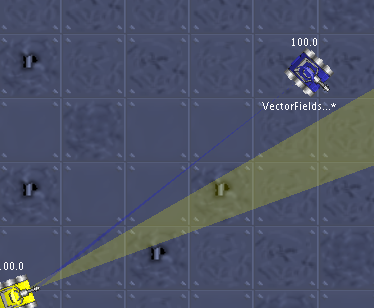
\includegraphics[width=0.5\textwidth]{images/RadarLock}
\caption{The blue tracking robot has located the goal with its radar, even though it is facing a different direction. It will never lose track of the goal now that it has a lock.}
\label{Radar Lock Example}
\end{figure} \\ \\
\noindent
To implement a radar lock that would never slip required simple algebraic manipulation of the state information present when an onScannedRobot event occurred. Whenever the goal was scanned, the radar's rotation was set to the tracking robot's heading added to the scanned ``goal'' robot's heading minus the radar's heading. More succinctly, $NewRadarHeading = RobotHeading + GoalHeading - CurRadarHeading$. This angle was then normalized so that it fell within the range of $[-\pi, \pi]$. This caused the radar to constantly rotate towards the direction that the goal was navigating so the radar never slipped and the goal was never lost. It also minimized the amount that the radar needed to be rotated so that less ticks were spent uselessly spinning the radar. \\ \\
Performance with the radar lock implemented was near as perfect as the simulation would allow. The robot could travel just as fast as the goal and never lose track of the location. In fact, the max speed of the tracking robot had to be turned down to ensure that it didn't catch up to and crash into the goal. In addition, because the tracking was so smooth, the speed of the bot could be appropriately scaled based on distance to the goal without fear of any blocking actions causing a loss of the goal or a slow scan resulting in a crash. \\ \\
Once the moving goal tracking had been sufficiently implemented, the next obvious step was obstacle avoidance. As with the goal, obstacles were nothing more than stationary or moving robot entities added to the simulation. The initial implementation of obstacle avoidance was simplified to include a single stationary obstacle and a stationary goal. This ensured that all issues with obstacle avoidance could be ironed out before dealing with the issues of adding a moving goal to the equation.  \\ \\
When a robot was scanned by the tracking robot that wasn't recognized as the goal, the robot would calculate and save the coordinates of that bot and assume it was an obstacle. Goal or obstacle recognition was handled in the onScannedRobot event handler by accessing the scanned object's name. The appropriate name values were simply coded into constants and checked whenever something was scanned. \\ \\
Since the location of the obstacle was stored as a pair of coordinates, the distance from the robot to the obstacle could be calculated during each iteration of the navigation loop. This distance value was checked against a previously defined threshold value that determined if the navigating robot was within the area of affect of the obstacle. The formula used to determine the repulsion from the obstacle was $\frac{Range - calcDist}{Range} * MaxSpeed$ where $Range$ was the threshold distance for the obstacle and $calcDistance$ was the calculated distance from the robot to the obstacle. $MaxSpeed$ was the maximum speed that the robot could be set to when running. This formula returned the amount that the robot's speed should be adjusted based on its location relative to the obstacle. This effectively slowed the robot down as it neared obstacles, which was necessary to ensure that it wouldn't cause a collision due to excessive speed in tight quarters. The direction of the repulsion vector was done using the \emph{archtangent} function like the goal implementation, except that the direction is from the obstacle to the robot so the ``force'' is repulsive. \\ \\
The next step was implementing a moving goal along with obstacle avoidance. Like the previous version with the stationary obstacle, the perfect radar lock could not be used because the tracking robot needed to scan for obstacles. Because it was planned that moving obstacles would be added in the future, a constantly rotating radar was used. While this may waste space over-rotating the radar, the trade off of perfect information for added situational awareness was both necessary and worthwhile. \\ \\
While the motion of the tracking robot was not nearly as smooth when a perfect lock was not used, the performance was still quite good. The motion was slightly jerky since a number of ticks pass before updating the goal position, but the obstacle avoidance worked well and the robot navigated cleanly. \\ \\
As a final test for potential fields, a reasonably complicated scenario with multiple obstacles, both moving and stationary, and a moving goal was constructed. Multiple obstacles meant that the code needed to be adjusted to handle the vector calculations in a general way. Because all the bots in the simulation could be given unique names by changing the class names in the implementation files, it was decided that a HashMap that mapped the robot names to instances of a class Enemy that held location data would be an efficient method for handling an unknown number of obstacles. 
\begin{figure}[htb]
\centering
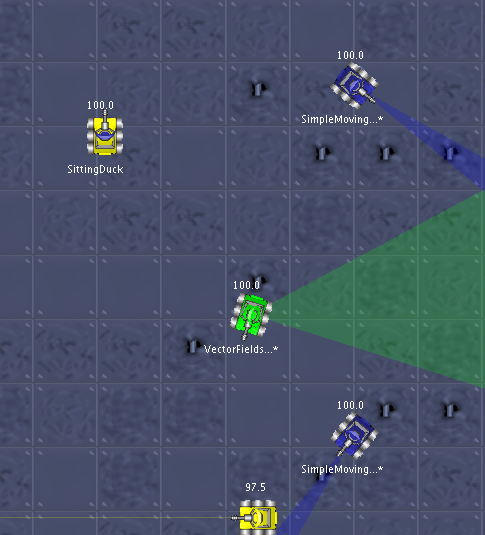
\includegraphics[width=0.8\textwidth]{images/FinalRun}
\caption{The final test for the Potential Field implementation features obstacles, both stationary and moving, and a moving goal.}
\label{Radar Lock Example}
\end{figure} 
\clearpage
\noindent
Each time the goal or an obstacle was scanned, onScannedRobot would grab the scanned object's name and insert an instance of the Enemy class into the HashMap. The Enemy class holds the calculated coordinate pair for the location of the scanned item as well as it's bearing at the time of the scan. The bearing was not used, but it was stored in case future modifications needed the additional information. This HashMap could then be iterated through in the navigation loop and the vectors could be calculated appropriately. \\ \\
The potential fields implementation handled the course beautifully. When it would pass between obstacles, its speed would be dropped sufficiently to avoid any near collisions. It also handled the moving obstacle quite well, so long as the obstacle buffer was set sufficiently high. If it was set too low, often times the robot would not react in time to sudden directional changes from the obstacles and would be crashed into. \\ \\
Perhaps the only change I would make to this algorithm would be taking into consideration how much to scale the speed based on how many obstacles are affecting the tracking robot. Each drop in speed was calculated independently for each obstacle. So if the robot was within range of three obstacles, each one of those obstacles would cause its own drop in the tracking robot's speed. This meant that often times the robot's speed would drop significantly even if it wasn't especially close to any one obstacle. However, the performance was still quite smooth with the current implementation. \\ \\
To finalize potential fields, it was decided that noise needed to be added to the model. Comparison really wouldn't be fair with the other methods if potential fields operated solely in an ideal environment. Noise was added in two ways. The first method added a random offset to the turning angle at a certain probability. As an example, twenty percent of the time the robot would slip $\pm 30^{\circ}$ when turning. The second method added small amounts of noise to the radar scans by adding or subtracting some $\epsilon$ from the calculated coordinate pair of the obstacle or goal. \\ \\
The potential fields implementations handled the noise quite well. The slips, even when really large, did not impact the results nearly as much as expected. Mostly the navigation path got a bit jittery, but the results were never catastrophic. Similarly, the robot didn't have too difficult of a time handling the radar noise. The noise was fairly small in comparison to the range of the obstacles, so there were not any collisions as a result of this. The only time the radar scan noise caused any truly noticeable effects was when the noise was turned up extremely high. So long as the noise was reasonable--$\pm$ a few percent of the total distance to the object--then the effect was not significant enough to cause problems.
% Conclusion
\subsection{Conclusion}
Overall, the potential fields implementation handled the majority of the situations it was put into quite well. Initially, the simple implementation worked as a proof of concept but not much else. It moved terribly slow, but it found the goal nonetheless. Moving over to a moving goal showed the weaknesses present in the simple motion model. It made it hard to constantly follow the moving goal. In fact, it was pretty much guaranteed that the tracking would fail unless the robot was started in the middle of the course and the goal robot travelled a specific path. Additionally, the speed of the tracking robot couldn't be scaled with regards to its distance from the goal without running the risk that it would lose track of the goal. \\ \\
The advanced motion model helped to smooth out the performance and addressed the issues made evident in the simple model tests. The radar locking experiment shows what the robot was capable of when it had perfect knowledge, and it showed the smoothest results when just dealing with a goal and no obstacles. It also demonstrated the speed adjustment with regards to distance from the goal best since it had perfect information on the goal. \\ \\
The obstacle avoidance results were quite good after the discovery of the advanced motion model. At first, expectations were low when watching the test runs with the simple motion model. However, the performance took off with the advanced motion model. Tracking a goal while dealing with an object was no challenge for the test bots. Even a moving goal with moving and stationary obstacles worked quite well. \\ \\
Even with all the successes, there were still problems present with the method. The implementations had difficulty with congested environments, especially when it would attempt obstacle avoidance too near to a wall. This was especially evident with high \emph{MaxSpeed} settings. Often times the robot would sweep wide around an obstacle that was near a wall and collide. Unfortunately, with Robocode it isn't possible to detect the wall with the radar. It would be possible to simply generate a repulsive vector based on the coordinates of the robot with regards to the width and height of the arena; however, that seemed a bit like cheating. Abusing the perfect world coordinates to the extent of making up readings didn't seem in the spirit of the tests. \\ \\
Additionally, the method struggled with closely placed obstacles since it couldn't detect the optimal path around them. This is where the planning of the other methods could become beneficial. The reactionary behaviour of the potential fields could be used to subsume the long term thought out behaviour present in the alternative methods. This could create quite a robust system.
\section{Markov Decision Processes}
\label{Markov Decision Processes}
\subsection{Introduction}
Markov Decision Processes (MDPs) enjoy widespread use today in the field of robotics. Roboticists have found MDPs to be particularly useful in the realm of motion planning. 
The primary reason for this is quite apparent: MDPs allow roboticists to generate optimal motion plans even in the face of noisy robot motion. Noisy motion is a fact of life for physical robots, so
the ability to plan optimally in face of that uncertainty is of incredible importance. \\ \\
The class lecture slides, the homework, the \emph{Probabilistic Robotics} textbook, and even the seminal \emph{Artificial Intelligence: A Modern Approach} textbook only considered MDPs in the context of static environments whose layouts were known \emph{a priori} to the
robot. This is obviously not a realistic assumption. Navigating robots must deal with situations in which the goal is moving, the obstacles in the environment are moving, or both. We wanted to investigate, in this part of our project, how effective MDPs could be in these types of online situations. \\ \\
More specifically, we wanted to investigate how well we could use MDPs in an online fashion to track a moving enemy robot in a simulated world. The effectiveness of MDPs in online contexts is obviously
closely tied to the efficiency and computational complexity of the method used to generate optimal policies in those MDPs. For this reason, we focused our observation and experimentation primarily on how well value iteration performed in online contexts and experimented with real-time extensions to value iteration that made it converge significantly faster than the full algorithm.
\subsection{Setup}
One of the first and most important things we had to do to set up this part of the project was to discretize the state-space. The Robocode battlefield is a $600 \times 600$, 2-D plane of continuous (x, y) coordinates. If we had made our state set equal to the set of (x, y) coordinates of the Robocode battlefield, our MDP state-space would have been infinite. Though MDPs can be applied to infinite state spaces, such MDPs would certainly not be suitable for the kind of online applications we had in mind. Thus, we decided to split the battlefield into equal-size grid squares, each of which became one state in our state-space. We chose a state space consisting of 400 $30 \times 30$ point squares. The choice of $30 \times 30$ grid squares was not arbitrary. Robocode robots are, in fact, very nearly this size. We devised a tiling function that associated any (x, y) coordinate with one of these 400 states. \\ \\
One other thing regarding the state space is worth mentioning. Usually, given an (x, y) plane with a moving robot, you need to include the orientation of the robot (with respect to some fixed frame) as part of each state. This is not the case in the Robocode world because Robocode robots are capable of turning immediately to any orientation at any time. In fact, we made heavy use of this capability in our action set. \\ \\
Next, we had to discretize the actions of the robot. Robocode robots are capable of performing a number of actions, the most important of which are as follows: move ahead some distance, move back some distance, turn gun some number of degrees, turn radar some number of degrees, and 
turn body some number of degrees. Each of these actions takes a floating point argument (for distance or degrees), so the action-space is also infinite. We knew that we would not be able to handle an infinite action-space in an online MDP, so we discretized the  action-space of the robot
as well. Since we were focusing on issues of motion planning, we decided to only consider movement actions as part of our MDP. Other necessary actions, such as sweeping the radar and firing the gun, were coded as purely reactionary or periodic. The robot swept its radar every 8 or so turns, and it fired straight ahead whenever it saw an enemy with its radar. \\ \\
Specifically, we discretized the motion action-space of the robot into 8 actions: goNorth, goSouth, goEast, goWest, goNorthwest, goNortheast, goSouthwest, goSoutheast. Each of these actions moves the robot ahead a static amount in the specified direction. We decided that going backward, though possible in Robocode, was an unnecessary complexity, because turning 180 degrees and going forward is the same thing as backing up.
\subsection{Implementation and Experimentation}
The implementation of the functionality for this part of the project proceeded in five main steps, each of which added additional complexity to the environment, the MDP test robot, or both. 
\subsubsection{Part I - Framework}
The first step we performed was to generate an MDP utility class (MDPUtility.java) that we could use for all of our MDP Robocode robot variations.
This involved developing, among other things, a simple reward function:
\begin{verbatim}
-100 for transitions from any state to the same state (hitting a wall)
100 for transitioning into a goal state.
-1 for all other actions	
\end{verbatim}
Next, we developed two different transition functions, one for noisy motion and one for non-noisy motion. The transition function for non-noisy motion is straightforward: each action in the MDP bot's action set takes the bot to one of the states surrounding its current state. For example, goNorth takes the MDP bot one state up (in the grid) and goEast takes the MDP bot one state to the right. Obviously, exceptions had to be made for the states surrounding the outside of the battlefield because some actions had the effect of keeping the MDP bot in the same state. \\ \\
The noisy transition function is similar to the non-noisy one but with the added complexity that the MDP bot has a 20\% chance of slipping each
time it takes an action.
More specifically, with a probability of 0.2, each action the MDP bot takes leads it the it to the state immediately to the right or left (from the bot's point of view as it is heading straight forward) of the intended state. This transition function was very tricky to build because of all the special exceptions that had to be made for the states surrounding the edge of the battlefield. For example, consider taking the action goNorthwest in the state at the bottom left corner of the battlefield. With no noise, this action has a 100\% chance of putting the MDP bot back in the same state. With noisy motions, there is now a 10\% chance that the MDP bot will head straight North into a valid state. All these possibilities had to be enumerated. \\ \\
Once we had finished these functions, we used them to code value iteration in Java. This gave us a basic framework we could use to begin exploring the use of MDPs in the Robocode world. In order to validate the above MDP framework, we performed the following steps:
\begin{itemize}
\item Picked a goal state on the Robocode battlefield arbitrarily.
\item Ran value iteration offline with non-noisy and noisy transitions and saved the policies produced by each run.
\item Created two simple policy-following robots (MDPTestBot.java and MDPTestBotNoisy.java in the provided code base), one for non-noisy motions and one for noisy motions.
\item Set a stationary enemy robot at the goal state.
\item Plugged the noisy policy into MDPTestBotNoisy.java and the non-noisy policy into MDPTestBot.java and verified that, from any random starting position, each of our MDP bots went directly to the goal state. 
\end{itemize}
We ran the above experiments a number of times with different goal states to verify our MDP framework. Below are the non-noisy and noisy optimal motion policies produced for leading our MDP bots to state 273. Each vector in these figures represents which action the robot is supposed to take in each state. States are numbered from 0 to 399, starting at the bottom left corner and proceeding row-wise up to the top right. You can see that, in each case (noisy and non-noisy), the policy produced leads the MDP bot to the proper goal state. The optimality of the policies is easier to see in the non-noisy one. Notice how the non-noisy policy has our robot making a direct line to the goal along the directions of our 8 motion actions.  
\begin{figure}[htbp]
   \centering
   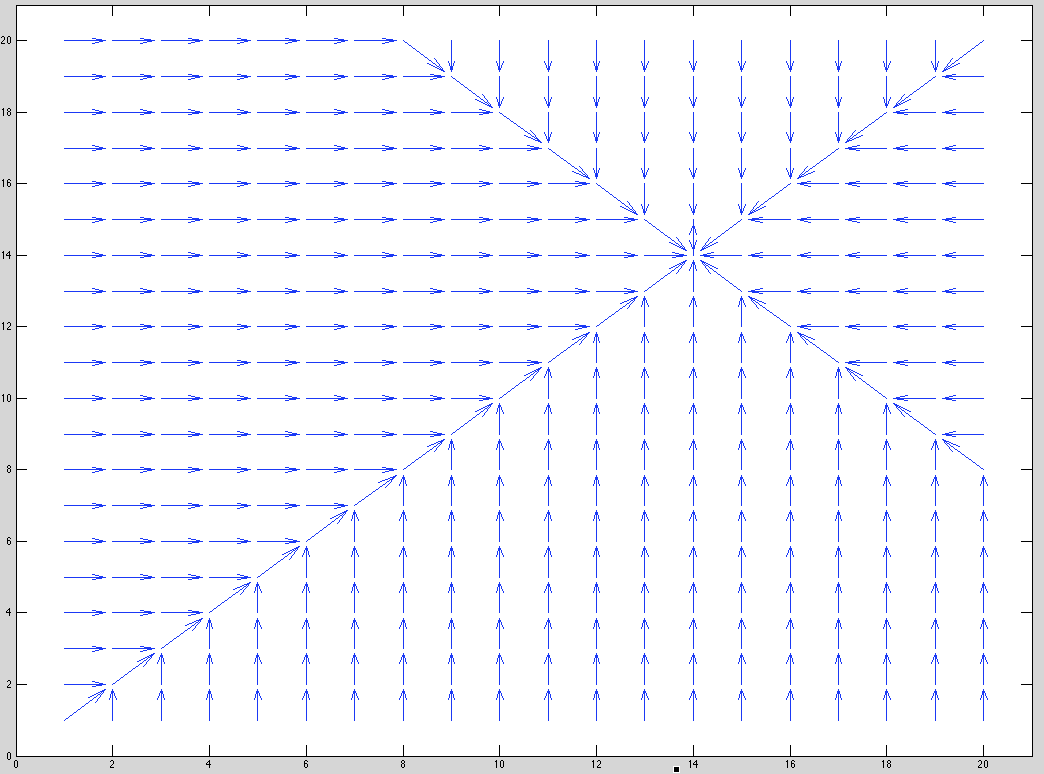
\includegraphics[width=170mm]{mdp_policy_to_state_273.png} 
   \caption{MDP Policy to lead an MDP bot to state 273. The motion of the MDP bot following this policy is assumed to have no noise.}
   \label{fig:sample}
\end{figure}
\begin{figure}[htbp]
   \centering
   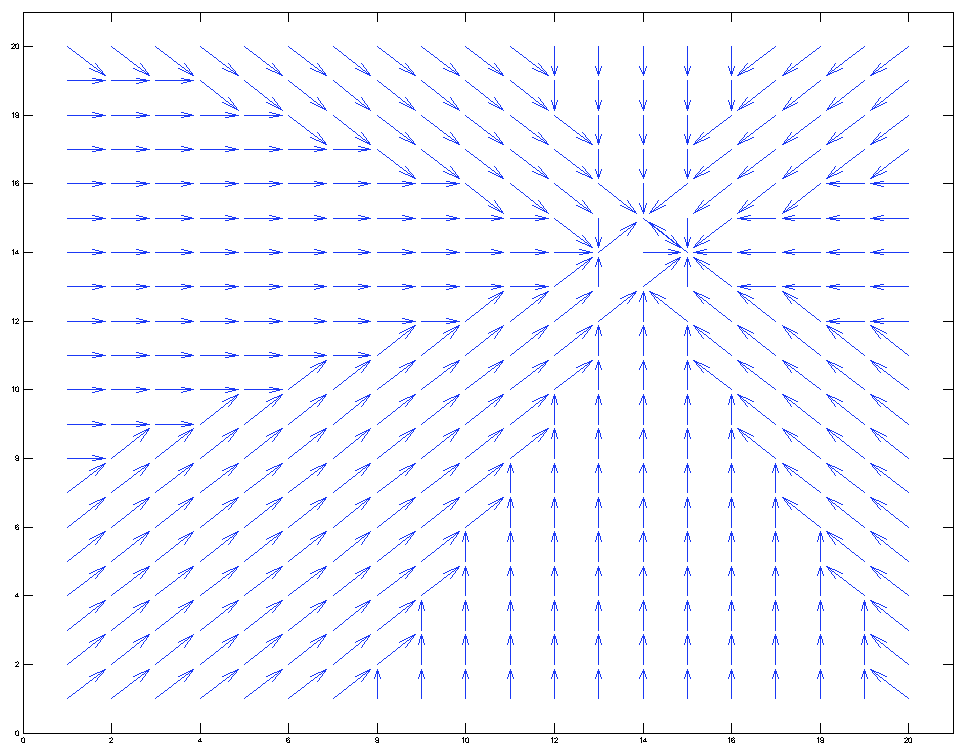
\includegraphics[width=170mm]{static_policy_noisy_to_state_273.png} 
   \caption{MDP Policy to lead an MDP bot to state 273. The motion of the MDP bot following this policy is assumed to follow the noise model described above.}
   \label{fig:sample}
\end{figure}
\clearpage
\subsubsection{Part II - Runloop Integrated Value Iteration}
The next main step we performed after developing and verifying our MDP framework was to find a way to run the value iteration "online" in the Robocode run loop. The first thing we tried was simply putting the value iteration function calls in the onScannedRobotEvent event callback function (triggered each time our MDP bot finds an enemy robot with its radar). This failed spectacularly because doing so blocked the main Robocode run loop of our bot. Our MDP bot was unable to take any actions during the time it was computing and was disqualified for skipping too many turns. We finally managed to integrate the full value iteration algorithm into a Robocode robot (MDPTestBotMovingTarget.java and MDPTestBotMovingTargetNoisy.java) by offloading the value iteration and policy calculations to a separate thread. We verified that we had successfully integrated value iteration into the Robocode run loop by doing the following experiment:
\begin{itemize}
\item Placed our MDP bot and the enemy bot in random locations on the map.
\item Had our MDP bot scan until it found the enemy bot.
\item Had our MDP bot calculate the (x, y) position of the enemy on the battlefield and find the corresponding state of the enemy robot.
\item Ran value iteration with the enemy's position state as our bot's goal state. This involved generating new rewards, a new Q-table, and a new policy.
\item Watched the MDP bot to make sure it went direcctly to the enemy position.
\end{itemize}
We performed the above experiment with non-noisy and noisy motion models, and we did it a number of times to make sure everything was working properly. This was a huge step toward our goal of running value iteration online with a dynamic environment.
\subsubsection{Part III - Moving Target Tracking}
The next step involved using value iteration online in order to follow a moving enemy bot. The implementation of this part was very similar to the implementation of the previous part, because we had already integrated value iteration into the Robocode run loop of a bot; however, there were a couple important changes we had to make to the code in order to make it follow a moving target. The most important change we made was to code in periodic radar sweeps. In general, generating a new policy through value iteration for a new goal state (new enemy position) took about 8 or 9 Robocode turns. So, every 8 turns we did a full 360 degree radar sweep of the battlefield to make sure that we had up-to-date information about the enemy's position. Before we added in the radar sweeps, our MDP bot was getting stuck forever at outdated goal states when the enemy took sharp turns. \\ \\
One interesting experiment we tried when developing this part of the code was predictive tracking. We tried running value iteration on the predicted goal state (based on the target's heading and velocity), rather than where the goal was when we started computing. We discovered that it was extremely difficult to estimate our own MDP bot's velocity because its motion is not smooth and because it continues following an outdated policy until the policy is updated. This made it almost impossible to estimate when we would reach the target position. We found that we got better performance with periodic radar sweeps and value iteration on the target's current position than with predictive targeting. \\ \\
 The experiments we did for this part essentially consisted of running our MDP bot against a number of different basic enemy movements and verifying that our MDP bot followed the target without veering off in weird directions or getting completely stuck. We found no cases in which our robot was unable to follow the target effectively. We did this with both non-noisy and noisy motion models and had success with both. The code for this step can be found in MDPTestBotMovingTargetDynamic.java and MDPTestBotMovingTargetDynamicN.java).
\subsubsection{Part IV - Moving Target Tracking with Real-Time Optimizations}
The fourth step of this part of our project was where we experimented with "real-time" value iteration. As was mentioned above, the full value iteration algorithm took about 8 Robocode steps to converge. This is obviously not ideal because, in the time it takes to generate a new policy, the MDP bot has already taken 8 turns worth of non-optimized actions (not necessarily 8 distinct actions because, in Robocode, you can have a velocity of 8 points/turn at a maximum). We wanted to significantly cut down the time our MDP bots were following an outdated policy.  Thus, we implemented what we are calling real-time value iteration. Real-time value iteration essentially performs a local value iteration update on the following states: the previous enemy positon (old goal state), the new enemy position (new goal state), the states surrounding the old goal state, the states surrounding the new goal state, the states surrounding the states surrounding the old goal state, and the states surrounding the states surrounding the new goal state. \\ \\
The intuition behind this update is that, if we are close enough to the enemy robot, and the enemy robot has moved very little since we last saw him (i.e., the distance between the old goal state and the new goal state is very small), we need only update our MDP bot's policy in that area of the state space to optimally lead the bot to the new goal. As long as our MDP bot stays in that updated area, it will be following an optimal policy to the new goal state. \\ \\
Specifically, the real-time update works as follows:
\begin{itemize}
\item We update the reward values we have for the new enemy position (new goal state), old enemy position (old goal state) and two layers of states surrounding each of these states.
\item We run value iteration only over the states for which we updated reward values to update the Q-values for the states we are updating. The key to the effectiveness of this part is that we do the Bellman backup only over the states surrounding the state being observed, because we can only move to a state from the states surrounding it.
\item We use the updated Q-table to update the current policy to reflect new actions in the states we updated. 
This produces a policy that is locally optimized for the new goal state (in the area we updated) and optimized in all other parts for the old goal state. Here is an example of what an updated policy looks like graphically. The goal state was moved from state 190 (dead center in the quiver plot) to state 150 (two states down from state 190). In this figure, you can clearly see how the policy is optimized locally for state 150 (in a 5 by 9 rectangle around states 150 and 190), but globally for state 190. In particular, observe how the diagonal lines in the four corners of the plot are headed straight for the middle of the plot (state 190). This policy, for clarity purposes, is for a robot with non-noisy motion. However, the real-time update works equally well with noisy motion models.
 \begin{figure}[htbp]
   \centering
   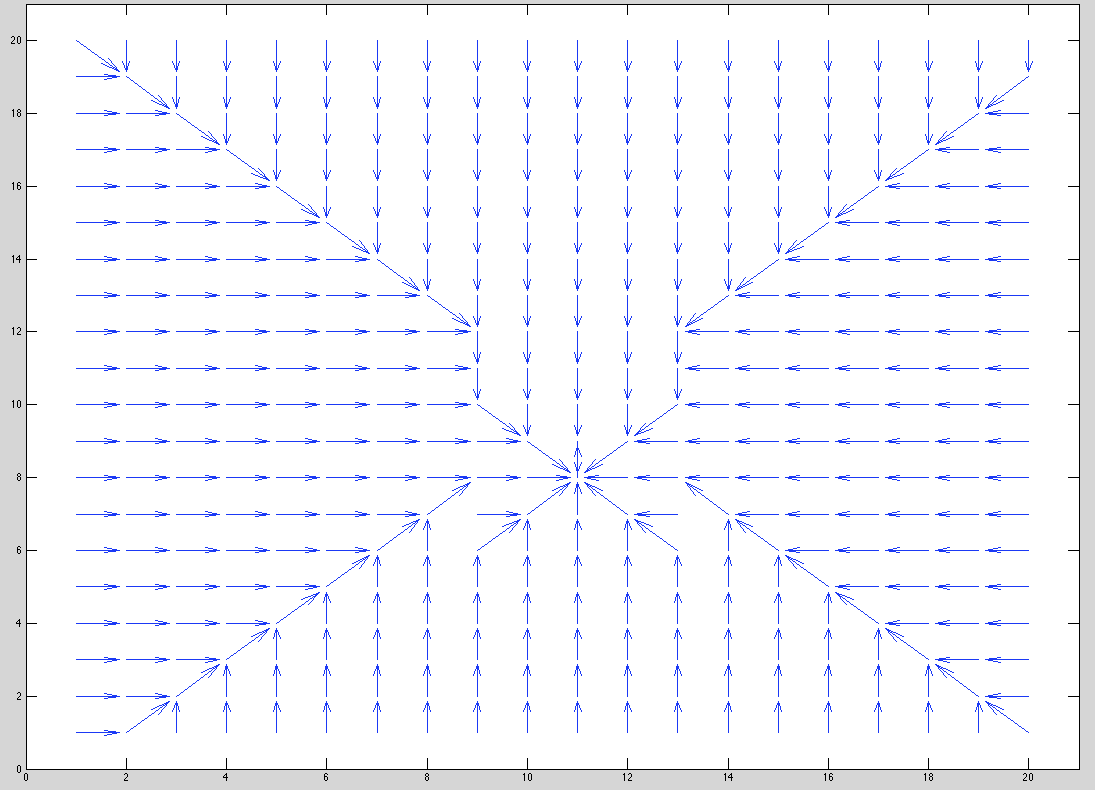
\includegraphics[width=170mm]{mdp_update_190_150.png} 
   \caption{MDP Policy that has been updated from goal state 190 to goal state 150 using our real-time value iteration function.}
   \label{fig:sample}
\end{figure}
\clearpage
\end{itemize}
We tested this procedure both offline and online. First, we tested it offline by running the full value iteration algorithm on a goal state, then running real-time value iteration to update that goal state. We saved both policies and verified that the latter policy was indeed a valid update of the former policy. 
Once we had tested this procedure thoroughly offline, we integrated it into new test bots (MDPTestBotRealTime.java and MDPTestBotRealTimeNoisy.java). Essentially, in these bots, we ran full value iteration to generate an initial policy and full value iteration every time the enemy was greater than 150 points away from our MDP bot. Once our MDP bot got within 150 points of the enemy, it transitioned to using the real-time value iteration update. The motion of our robot when it gets close to the enemy bot is noticeably more fluid in these bots because the real-time value iteration function converges in 0 Robocode turns. Our MDP bot is thus able to calculate an updated policy and start following that policy in the same turn. We ran this online, real-time experiment with a number of different enemy bot motions and with both noisy and non-noisy motion models. \\ \\
We saw some noticeable improvements to enemy tracking with the real-time value iteration algorithm when our MDP bot was close to the enemy bot, even when the MDP enemy bot made sudden changes in direction. However, as was mentioned before, when the old goal state and the new goal state are too far from one another (perhaps because the enemy slipped out of our radar view for a few turns), the real-time update function fails, and the robot appears confused until it has time to do a full value iteration update. Consider the following figure. Here we have updated a policy from goal state 25 to goal state 31. Notice how all of the actions surrounding the old goal state have defaulted to going North. The new goal state is too far away from the old goal state to pull the actions around the old goal state in the direction of the new goal state. This is the major limitation of the real-time value iteration algorithm, and it is the reason we only used it in our MDP bots within a certain range. Based on our empirical evaluation of the real-time value iteration function, 5 states is as far of a jump as you can make (between old goal states and new goal states) without this improper behavior occurring around the old goal state. Again, for clarity, this figure is a policy for a noise-free motion model.  
 \begin{figure}[htbp]
   \centering
   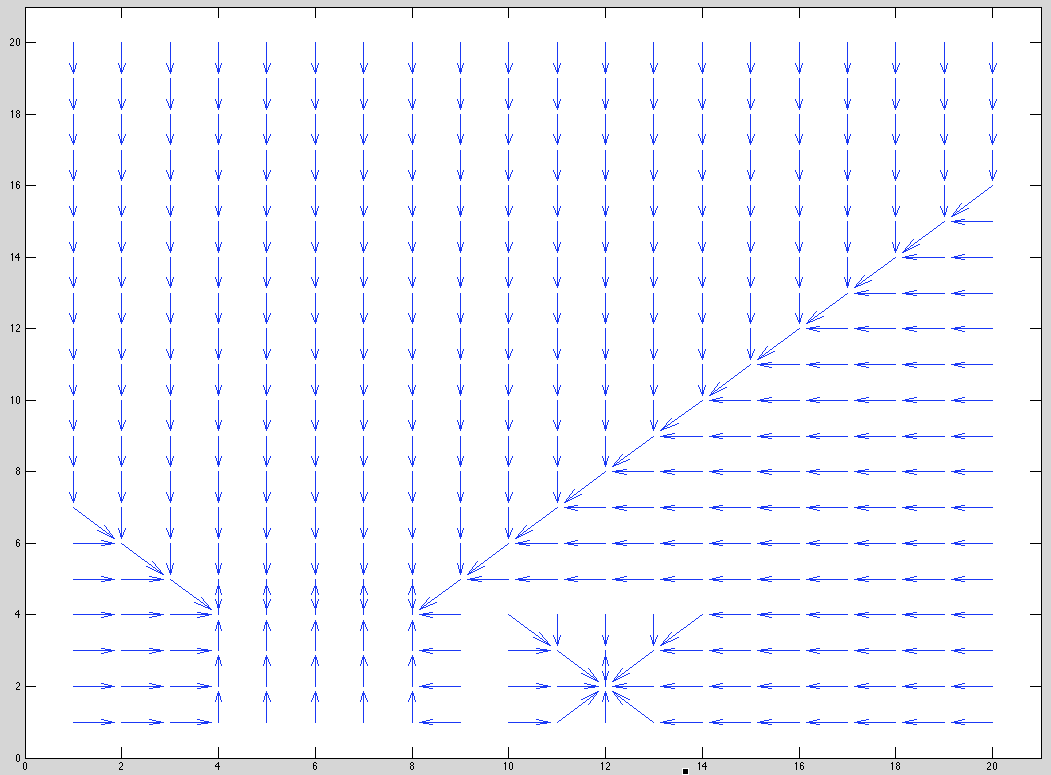
\includegraphics[width=170mm]{mdp_policy_update_25_to_31.png} 
   \caption{MDP Policy that has been updated from goal state 25 to goal state 31. With this large of a jump between goal states, the real-time value iteration algorithm fails.}
   \label{fig:sample}
\end{figure}
\clearpage
\subsubsection{Part V - Dynamic Obstacle Avoidance}
The fifth and final major step we took to implement MDPs in dynamic Robocode environments was to add in support for obstacle avoidance (moving or stationary obstacles). In the context of the Robocode environment, obstacles are simply other robots on the battlefield that we are not tracking. This was a major update to our current MDP bots because none of them had yet considered more than one other robot on the battlefield. We ended up representing these obstacles as a hash map. In Robocode, when a robot's radar discovers another robot, the name of that other robot is returned. Each of these names is guaranteed to be unique in the given battle. We used this name as the key of the obstacle and saved its current state as the value. We knew the name of the enemy we were tracking before the battle started, so we were able to distinguish this bot from all of the other bots. Every time we saw the same obstacle again, we updated its value (current state) in the hash map. This representation allowed us to track a list of obstacles (of arbitrary size) and their movement over time.  \\ \\
In addition to tracking objects and their positions over time, we had to factor them into our reward function. We wanted to ensure that this reward function made getting close to an obstacle bad enough that we avoided obstacles, but not so bad that we didn't risk going anywhere near them to track the target. We settled on the following updated reward function: 
\begin{verbatim}
-100 for transitions from any state to the same state (hitting a wall)
100 for transitioning into a goal state.
-20 for transitioning into an obstacle state
-20 for transitioning into a state surrounding an obstacle state
-20 for transitioning into a state surrounding a state surrounding an obstacle state
-1 for all other actions	
\end{verbatim}
These rewards make our MDP bots tend to avoid going within two states of obstacles on their way to the goal state. It is a very conservative reward function in the sense that it makes the MDP bot give itself a large buffer around obstacles. We also tested obstacle avoidance both offline and online. For our offline tests, we added obstacles to a hash map and ran value iteration with the new reward model to ensure that our policy was indeed pushing us away from the obstacles we specified and still leading us toward the goal. We tried this with different numbers of obstacles and obstacles in different locations. \\ \\
 Once we were certain that was working, we integrated the obstacle avoidance reward structure and policy generation into new MDP bots (MDPTestBotDynamicOb.java and MDPTestBotDynamicObNoisy.java) and verified that obstacle avoidance worked in an online fashion. We tested our bots online with stationary obstacles and a stationary goal, stationary obstacles and a moving goal, a stationary goal and moving obstacles, and moving obstacles and a moving goal. In each test that we ran, it was readily apparent that our MDP bots were both avoiding the obstacles on the map and still heading toward the goal state. \\ \\
It is also worth mentioning one behavior that we noticed of these MDP bots. If the MDP bot tried to run value iteration when the goal robot was within one or two states of an obstacle, the MDP bot would just head straight North until it was able to see the enemy bot again a safe distance from any obstacle. We ran this test offline and verified that almost all of the actions defaulted to North in this case. This behavior makes sense. It is quite obvious that the MDP bot was unable to find a path to the goal that was not too painful reward-wise. It didn't know anything better to do, so it defaulted to going North in most states. Below you will find two figures. The first figure is a graphical representation of a policy that avoids two obstacles and leads to a goal. The second figure is a graphical representation of the policy produced when the goal-obstacle proximity problem described above is encountered. Both policies are for MDP bots with the noisy motion model described above.
 \begin{figure}[htbp]
   \centering
   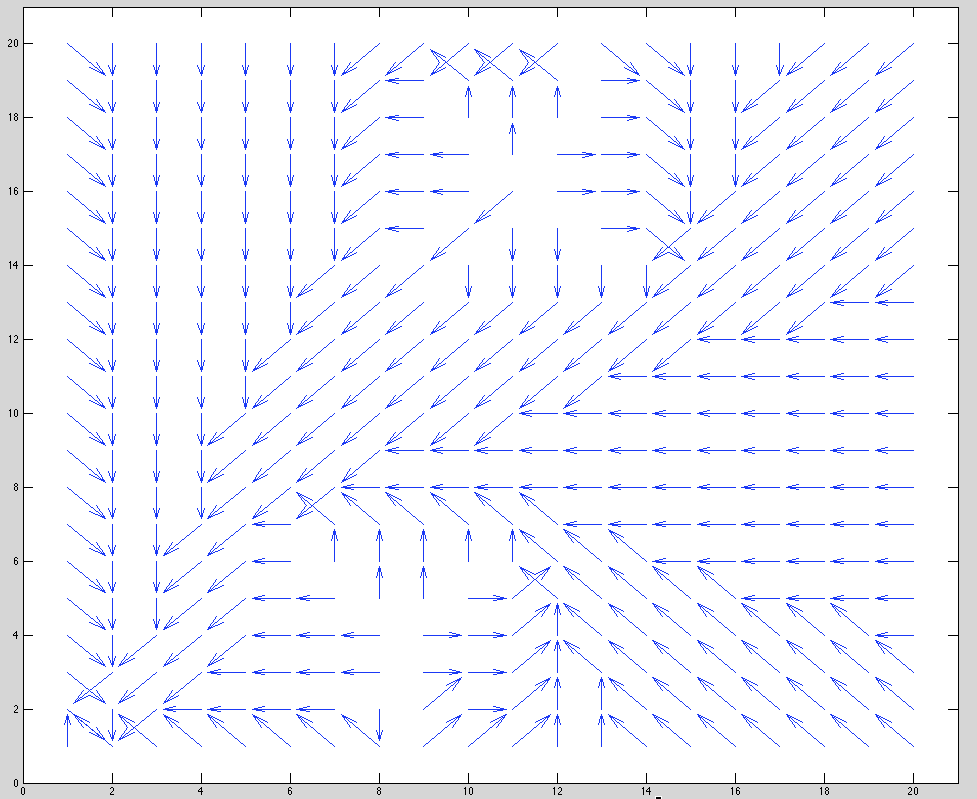
\includegraphics[width=170mm]{mpd_noisy_obstacles.png} 
   \caption{MDP Policy to lead an MDP bot to state 0 while avoiding obstacles at states 67 and 310.}
   \label{fig:sample}
\end{figure}
 \begin{figure}[htbp]
   \centering
   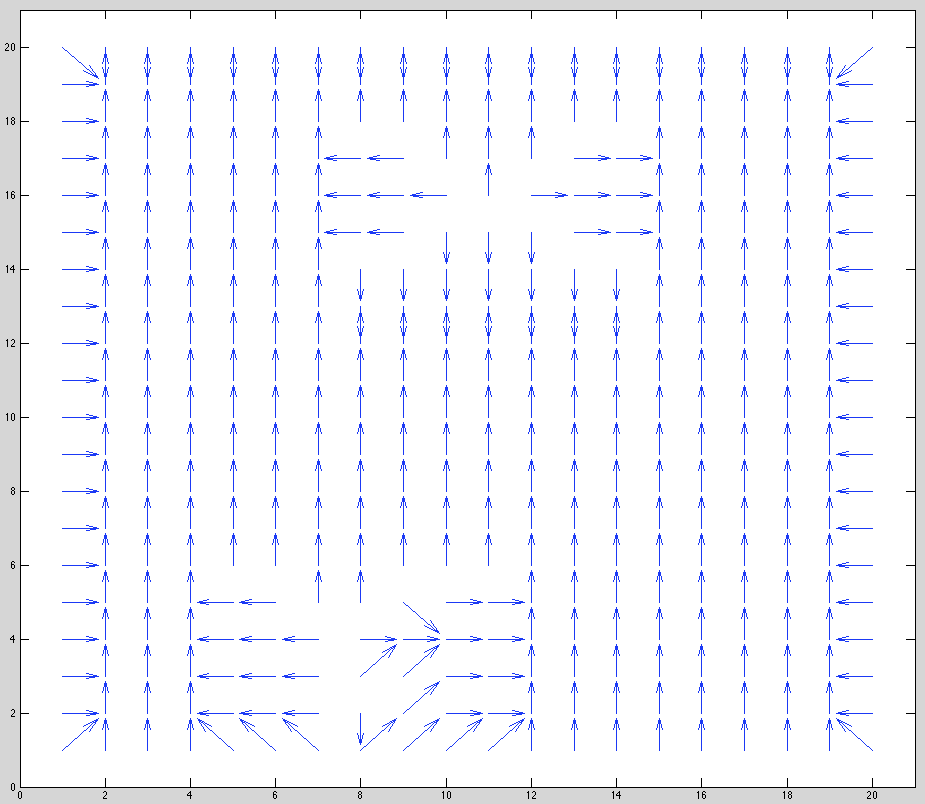
\includegraphics[width=170mm]{mdp_proximity_error.png} 
   \caption{MDP Policy to lead an MDP bot to state 68 while avoiding obstacles at states 67 and 310. The goal state is too close to the obstacles, and the path to the goal is obliterated.}
   \label{fig:sample}
\end{figure}

\clearpage
\noindent
As a final experiment, we attempted to code a real-time value iteration update that took obstacles into account. We took the real-time value iteration algorithm that we had built and modified it to also update the old and new states of the obstacles in the environment, as well as the states in the two rings surrounding the old and new states of each obstacle. Though we were able to get this function to converge in fewer iterations than the full value iteration algorithm, the results were non-intuitive. We speculate that perhaps the obstacles were too far away from the goal to update the obstacle locations in a way that was reasonable. There is also a possibility that the code itself is erroneous.
\subsection{Analysis}
In the Robocode environment, we were able to successfully implement a number of MDP bots that allowed us to examine the effectiveness of MDPs as a motion planning paradigm in different online motion planning and tracking contexts. In the preceding experiments, we discussed many of the things we learned about utilizing MDPs in an online way and many of the problems we encountered in doing so. In general, we found MDPs to be effective (in the sense that they successfully did what we wanted them to do) but relatively slow. This came as no real shock to us. Consider the computational complexity of the value iteration algorithm, particularly the inner loops. Let $s$ be the number of states and $a$ be the number of actions in the MDP. The computational complexity of these inner loops is $\Theta(s^2a)$. This clearly does not scale well as the number of states and actions increases. This computational complexity must also be multiplied by the number of times the outer while loop runs. For our MDP setup in the above experiments: 400 states, 8 actions, a 0.9 discount factor, and a Bellman residual of 0.01, it took 114 iterations of this outer while loop for value iteration to converge (116 iterations for the noisy motion model). Lower Bellman residual values caused this number of iterations to balloon. This is why the MDP bots we created were relatively slow to react to sudden changes in enemy position and obstacle position. The MDP bot had to consistently follow an outdated policy for several turns before it figured out how to get to the new goal. If the enemy took a sharp turn and moved at the maximum rate of 8 points per Robocode turn for 8 turns, it could be 64 points (about 2 states) away from the last place our MDP saw it before our bot figured out that it needed to turn and go a different direction. This accounts for the lack of fluidity in the MDP full value iteration tracking performance we saw and the relative ease with which our MDP bot lost track of the target when the target took sharp turns. On the other hand, full value iteration still worked surprisingly well. The full value iteration MDP bots we built do a decent job of following the target, even in the face of obstacles, provided that the MDP bot moves at least as fast as the enemy bot. Though 8 turns worth of suboptimal MDP bot action is clearly not ideal, it was not enough time for the enemy to get so far away that our MDP bot could never catch up again.  \\ \\
Still, we were unsatisfied with the performance of the full value iteration algorithm. One of the goals of our project was to make MDPs work in real-time. This meant that the MDP robot had to be able to update its policy \emph{and} follow that new policy in the same turn. In order to do this, we needed to find a way to boil down the aforementioned  value iteration algorithm to essentially a constant operation. The algorithm we developed, the specifics of which are discussed above, does a local policy update on 50 states: the new goal state, the old goal state, and the states in the two rings of states surrounding each of the old goal state and the new goal state. This algorithm creates a locally optimized policy for the new goal state and leaves the remainder of the policy optimized for the old goal state. If the old goal state and the new goal state are close together, this generates a global policy that can best be described as nearly or approximately optimized for the new goal state. Though this method is probably most useful in situations in which the MDP bot is very close to the enemy (which is how we made use of it), it could theoretically be used successfully at large distances. The beauty of this method is that it converged in 0 Robocode turns. It is therefore a full-fledged real-time value iteration procedure, at least for our (admittedly) small state-space and action-space. Notice that, though this is a constant operation with regards to state-space, increasing the size of the action space does affect the running time of this algorithm. As was mentioned above, this algorithm noticeably increased the smoothness of our MDP tracking when our MDP bot was close to the enemy and the enemy was within the radar scope of our MDP bot. With the completion of this method and the introduction of obstacles as a stress test, we had accomplished everything we set out to do in the MDP part of our project and gathered some great results.
\section{Q-learning}
\label{Q-learning}
\subsection{Introduction}
Reinforcement learning is generally more computationally expensive,
less fine-grained, and less deterministic than other methods we've
examined. Given these obvious downsides, especially in a
real-time dynamic context, why is this approach worth
considering? Primarily, it brings the potential for a great deal of
flexibility in handling unknown environments, sensor quality, and
motion models. While, if other methods are possible, they should likely
be the first choices, it does provide a valuable option in certain
cases. 
\subsection{Setup}
The basic Robocode setup for Q-learning extends
the setup for MDPs. The basic methods of discretizing the state
space, discretizing robot movements, and handling the threading needed
for long-running processes were similar between the two methods. \\ \\
Given the structure of the algorithm, the large transition tables of
the MDP approach were not required. The noise could be added on each movement
step during training and actual runs. As such, all we required was a
basic randomization method to send the bot on an incorrect path a
certain percentage of the time. This was kept the same as in the MDP
tests with an 80\% probability of following the selected route with a
10\% chance of slip with motion along either of the two adjacent
movement directions. \\ \\
Basic rewards were structured similarly to the MDP trials. An action
which led into the goal state returned a reward of 100, an action
which caused motion into a
wall (or, later, an obstacle) gave a -100 reward, and all other
actions returned a reward of -1. \\ \\
For policy visualization, we wrote a method in Matlab to take the output
policy and convert it into a quiver graph which proved useful for
visualization of all discrete policies.

\subsection{Experiments}

\subsubsection{Offline trials}
The first step was to confirm the functioning of the basic
Q-learning method. To do this, we ran initial tests with a fixed
starting point for the bot and a fixed, stationary
goal. The learning was run offline, a policy generated and
incorporated into a simple bot whose only processing was to determine
its current state and run the appropriate policy. \\ \\
Initially these tests were run in a noiseless environment to
confirm basic operations of the various components. Adding in noise
produced distinctly rougher bot motion, but did not impact the overall
effectiveness of the method. \\ \\
Both Boltzmann explorations and $\epsilon$-greedy were experimented
with at this phase.  We began by exploring the quality of the policies
given an equal numbers of trials. Here Boltzmann was clearly
superior, producing policies which more consistently and directly led
to the goal. \\ \\
But the constraint was on computational time, not episodes so we
further ran a series of rough tests comparing along this axis. $\epsilon$-greedy method ran in approximately half the
time for a given number of trials (a ratio which seemed to scale). So, at this point, we compared $\epsilon$-greedy
with twice the number of trials against Boltzmann. Even in this case,
the overall policy produced by Boltzmann was better with fewer failure
incidents and better tracking performance. While both were left in as options on all future
bots, Boltzmann was the default from this point on. The advantages in
overall performance and quality per unit of computational effort were
clear.
\subsubsection{Taking it online}

Things became a bit more complex as we shifted to
learning in the context of the environment itself. This required
several basic elements. First, the bot required the ability to scan
the environment for the location of the goal state. Second, the bot
required the ability to call out to the Q-learning method from inside
the Robocode environment. Finally, there needed to be a default policy
for the initial period when the bot had not yet learned a policy given
the environment.  \\ \\
The most difficult part of this was dealing with a long-running
learning process in the context of the Robocode environment. As we
discussed in the MDP section, this was accomplished by spawning a
separate thread to run the learning process while a default random
policy was executed as the robot continued to scan the field. \\ \\
For initial testing, we started the bot and goal in fixed points so
that we could control for the starting conditions. However, we were
quickly able to transition to randomly placing the two elements. The overall
performance on these tests was good. The bot could randomly move while
calculating its policy and then shift over to the resulting policy
once complete.
\subsubsection{Performance and dynamic environments}

At this point we shifted over to allowing for motion in the goal
state. Several issues became apparent at this point. The first was that, as we'd expected, the
speed of Q-learning was an issue in a dynamic environment. The numbers
of episodes we'd run in the offline tests or even in the
static tests were no
longer feasible.  \\ \\
The first thing we tried was lowering the number of episodes. 
However, this produced policies of a noticeably lower quality. In
particular, the bot had a tendency to get caught in state loops where
an incompletely learned policy would have two states which pointed to
one another. The other primary failure mode were states which directed
the bot directly into a wall. \\ \\
While the number of episodes traded off fairly directly with
the quality of the policy, we were not able to implement a
precise way of tuning this relationship. We settled on 100,000 episodes as a manageable
compromise. While not producing perfect policies, it generally ran in under two
seconds (often closer to one) which was essential to
keeping tracking reasonably accurate. This would clearly be an area
for more detailed future exploration. \\ \\
However, even that shortened learning time imposed a cost on the process. Notably, in
that period of time the bot (and, in later experiments, the goal)
could have shifted location rather dramatically. Several pieces were
added to attempt to account for this. \\ \\
First, we added a basic predictive aspect to the location of the goal
state. This meant accounting for its current velocity and bearing and
predicting where it would be after the policy was completed. However,
there were a number of issues with this method. The prediction itself
needed to account for the structure of the environment (walls, in
particular). Additionally, changes in direction by the goal could make
this approach directly maladaptive. While we kept experimenting with
this, past a certain point adding too much intelligence to the
prediction seemed to defeat the aim of the learning agent. Still, in
limited contexts this was a useful tool. \\ \\
Second, we added a more robust method for recalculating policies. The
first method that was tried was recalculating each time the goal
was viewed. Simple locking was put in place so a new update thread was
only spawned if an update wasn't currently in progress. The downside
to this method was that it was precisely at points when the goal
hadn't been seen lately that an update was most necessary. \\ \\
So, we extended this to keep track of the last view of the goal and, if
that passed a certain count of turns to pause, scan the field for the
goal, and then learn a new policy. However, what proved best was to
simply always be recalculating the policy. Effectively, each time a
policy was produced, the goal would be scanned for and a new learning
process begun with the current location of bot and goal. \\ \\
This led to the next major performance adjustment. In earlier trials,
we had attempted to learn a whole-field policy since, with a single
learning cycle to work with, we had to have as universal a policy as
possible. To accomplish this, starting positions of the bot were
randomized from episode to episode in order to maximize coverage of
the state space. \\ \\
At this point, we shifted to focus the start position
on the current location of the bot in relation to the goal. The upside
of this was to produce policies that were generally more effective
given a limited number of learning episodes. The downside was that
failure modes were far more severe when entered. As can be seen in the
following policy areas away from the primary route from bot to goal
were nearly unlearned.
\vspace{.3in}

\begin{figure}[htbp]
  \centering
  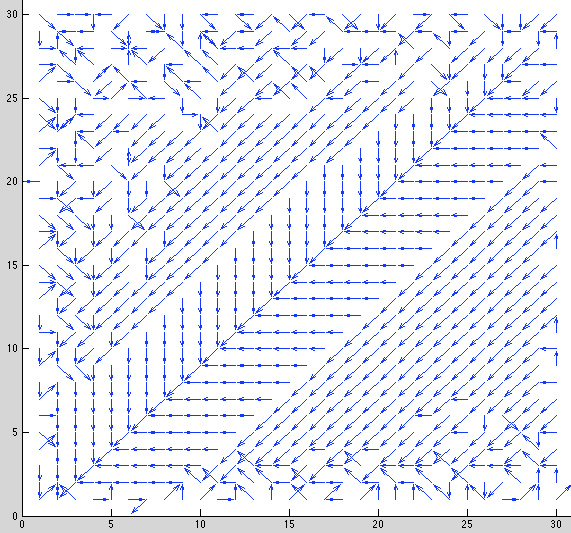
\includegraphics[width=\linewidth]{images/BasicPolicy.png} 
  \caption{Basic Q-learning generated policy.}
  \label{fig:basicQ}
\end{figure}
\clearpage
\begin{verbatim}
\end{verbatim}
However, frequent updates proved an effective antidote to these
issues. In most cases, even when the robot was caught in a loop of
states, the next update would free it to continue tracking the goal.

\subsubsection{Obstacles}
The final major addition we made was to add obstacles to the
environment. In the first iteration of this, these were fixed and
pre-specified environmental features. At the next phase we moved to
allowing dynamic obstacles in the environment which the bot had to
scan and incorporate into its model. \\ \\
The changes required to support this weren't huge. The bot had to be
capable of distinguishing obstacles from the goal and treating the two
differently. On the learning side, this required an adjustment to the
reward model to account for obstacles in the learning
process. We treated obstacles as equivalent to walls with a -100
reward for colliding with an obstacle. An example of a policy which
accounts for obstacles (in this case, a wall in the lower left quadrant) can be
seen below. 
\vspace{.3in}

\begin{figure}[htbp]
  \centering
  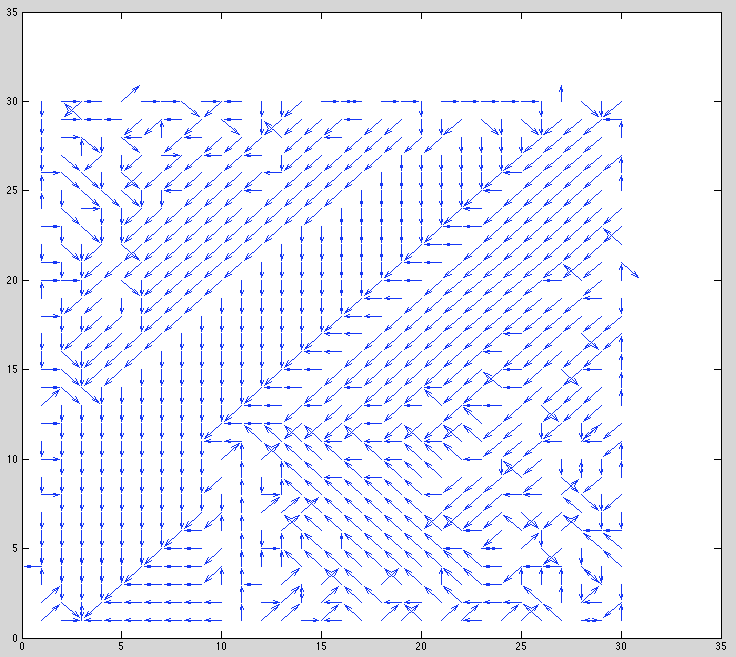
\includegraphics[width=\linewidth]{images/Wall2.png} 
  \caption{Q-learning generated policy with wall present at $x=10$.}
  \label{fig:obstacleQ}
\end{figure}
\clearpage
\begin{verbatim}
\end{verbatim}
There were several issues with this. The first was a slow-down in overall processing. We were unable to isolate the causes for this precisely, but handled it by adding threads (to the max supported by Robocode, five) and lowering the number of episodes in each cycle. This worked, but nonetheless the tracking performance was far from optimal. \\ \\
Additionally, obstacles could shield one
another, preventing the back one from being scanned. This was
generally not an issue as, by the time the second obstacle was
reached, a new scan had generally taken place. More issues were caused
by the fact that the goal could also be shielded by an
obstacle. For this, the best we were able to do was constantly update
the goal location so that, even if it was hidden by an obstacle prior
to a new learning process, we would still have a reasonable estimate
of its position. \\ \\
However, given all of the previous issues, moving obstacles proved
slightly too much for these methods. Beyond a certain amount of
complexity on the field, the updates were simply too slow to produce a
viable policy.

\subsubsection{Heuristic reward functions}
Finally, we explored replacing the fixed reward function with a
heuristic based on euclidean distance to the goal. For smaller numbers
of episodes, this produced much better policies. The reason is that,
given the structure we'd set up, this basically approximated a
search function. Effectively, at each step, it
would choose the step closest to the goal. For a single episode,
this would look like a depth-first search. In the simplified
environments we were working with, there would be little or no
backtracking required. Over a number of episodes, this would start to
look more like a best-first search, specifically A* given the use of a
valid heuristic function. \\ \\
Surprisingly, the results were not better for this method with a larger
numbers of iterations. What we observed were policies that actually
gave less complete coverage of the state space. This can be seen in
the following policy which can be compared to Figure~\ref{fig:basicQ} (same
start and goal locations).

\vspace{.3in}

\begin{figure}[htbp]
  \centering
  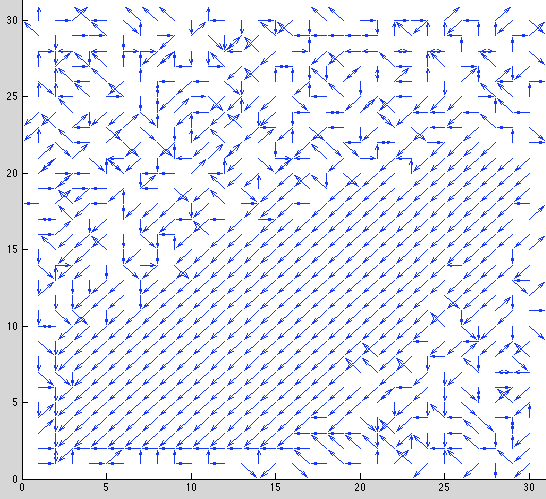
\includegraphics[width=\linewidth]{images/HeuristicPolicy.png} 
  \caption{Q-learning generated policy with a heuristic reward policy.}
  \label{fig:heuristicQ}
\end{figure}
\clearpage
\noindent
This may well have been a result of exploration
not being properly tuned to the improvement in the reward
function. The heuristic reward, in pulling each step towards a greedy
depth-first approach, would require a more powerful push to exploration
to overcome the additional pull of the new reward function. The lack
of this may have led to a failure to explore
the state space as widely. Of course, if this type
of reward and environment information were consistently available to an actual bot,
simply
running a true A* would be far more
efficient and could be updated in real-time for such a highly discretized
space.
\subsection{Evaluation}
While Q-learning had clear weaknesses in this context, we were able to take it farther towards a real-time context then we expected. Additionally, our exploration of heuristic reward functions pointed to an interesting tension between information and exploration. We look at these issues in detail below. \\ \\
The largest issue with our implementation of Q-learning is that it
relies on information which, if present, could better drive a more
efficient and/or complete method. By pulling information about the
field into what amounts to a local simulation in which the learning
takes place, we undercut much of the real-world justification for the
use of a learning method. However, our aim was to consider these
methods primarily for future use (Robocode, while charming, is not the
end goal). In that context, our results suggest certain
more interesting possibilities. \\ \\
In addition to the expected downsides: slow update time, non-optimal policies, and risk of being caught in
local state loops, Q-learning also proved somewhat brittle, in
many cases failing completely. This seemed to be an interaction with
the Robocode environment. For example, when an incorrect policy would
have the bot repeatedly attempt to push through a wall, Robocode would
disable the bot. \\ \\
However, the more surprising
result is that we were able to get Q-learning running well-enough to
successfully operate in a dynamic real-time environment at all. The
fact that policy updates could be recomputed fast enough to
maintain tracking on a moving goal was interesting and somewhat
surprising. We'd expected that this method would have to be used
largely offline with policies generated and fed in. Being able to get
it to the point of updating while in a dynamic environment was a surprise. \\ \\
In particular, this suggests several ways that Q-learning might serve as a
component of an overall navigation system. One possibility would be as
part of an overall voting system. Especially given a noisy
environment, a learning method could provide a needed bias among
competing focused heuristics. \\ \\
A better approach would likely be a hybrid system. For example, say
there were a number of different standard goal movement patterns, but
these were obscured by uncertainty in motion, shifting environmental
conditions, etc. A learning method combined with more straightforward
predictive modeling of the other bots could potentially help to
account for that noise. Action choices would still be managed through
more efficient methods, but the choice among those methods handled by
a learned evaluation over a given set of state parameters. \\ \\
One area where more work is definitely needed is on reward function
optimization. Clearly there is a great deal of tweaking and rebalancing
possible, but we were not able to fully explore the implications of
this. \\ \\
However, our experiment on shifting from fixed rewards to
heuristic rewards provided some interesting hints as to future possibilities. First, the hidden cost of
adding information into the reward in terms of overwhelming the
pressure to explore was not something we expected. The difference in the size of the explored portion of the field was clear both in extracted policies (see Figure~\ref{fig:basicQ} and Figure~\ref{fig:heuristicQ}) and in actual bot performance. \\ \\
It
emphasized the need for improved reward information to be combined with a greater emphasis
on exploration. Uncertainty in the system (from both sensors and
motions) has to be reflected in the learning process. In particular, a reward function that pulls the bot too strongly towards the goal will need to be balanced by a stronger tendency towards exploration. However, the precise nature of this balance depends a great deal on the structure of the situation and what level of generality is required from the policy. \\ \\ 
Additionally, it
suggested some interesting possibilities in terms of injecting
additional information into learning methods as a way to take
advantage of additional information if present. This might be
especially useful in a situation where such information were only
sporadically present. For example, a noisy sensor which sporadically
gave a distance measure could be incorporated, but with the awareness
that additional weight might need to be given to exploration to
balance this out in a learning context. \\ \\
The central theme in our exploration of Q-learning in a dynamic
context was one of tradeoffs. While this and related reinforcement
learning methods are extremely powerful and flexible (most of that power
left untapped in this case), the tradeoffs involved in their application require an awareness on the part of the designer of both the overall structure of the problem and what is desired from their resulting policies. More, it 
seems to suggest their ideal use might be in combination with other
methods. Applied properly, those strengths can be exploited while the weaknesses
are shored up by other methods.
\section{Conclusion}
\label{Conclusion}
\noindent
Potential Fields performed quite well in the Robocode environment. Combining the advanced motion model with the potential fields approach allowed for smooth navigation and obstacle avoidance. The potential fields method was quite robust and handled changes to the environment better than either of the other two methods. The primary performance limitation of potential fields was the speed with which the environment could be scanned with radar sweeps. The navigating bot's max speed and obstacle avoidance radius had to be tuned with the radar in mind. Even so, the robot was able to navigate fairly complex environments. \\ \\
Of course, that isn't to say that potential fields didn't have problems. Suboptimal navigation is always an issue that potential fields will have. This became especially true when obstacles were placed really close to the walls since the radar sweeps didn't read the distance to the walls. It would also rather avoid close obstacles than navigate between tight paths, which may not always be optimal. There is also the issue of local minima causing navigational issues. That being said, potential fields handled the environment quite well. \\ \\
Markov Decision Processes (MDPs) also proved to be a decently effective framework for enemy tracking in dynamic Robocode environments. Though generating new, optimal policies took a number of Robocode
turns, we were able to minimize the effects of this policy lag through clever use of multithreading in the Robocode run-loop and periodic radar sweeps. Though the resulting tracking was neither perfect nor very fluid,
we did achieve our primary goal for integrating MDPs into our project: we successfully used them in an online context to follow a moving target, even when the environment contained an unknown number of moving obstacles and the initial position
of the goal was unknown. \\ \\
The most important aspect of the MDP part of our project was undoubtedly the real-time value iteration procedure that we constructed. By considering only the area surrounding the old and new goal position, we were able to update our MDP policy and follow
that updated policy in the same turn. In the context of the Robocode world, this constitutes a real-time update. With the completion of this aspect of the MDP part of our project, we had completed our secondary goal of using MDPs online in Robocode in real-time. We verified this
procedure with rigorous offline and online testing, and the results were quite exciting. We saw very smooth tracking by our MDP bots when we utilized this real-time update at close proximity to the enemy.\\ \\
Q-learning proved to be the least effective method of interacting
with the dynamic Robocode environment. The extra processing required for the generation
of new policies left the robot lagging well behind the goal in most
situations and occasionally led to it to being caught in unlearned
segments of the policy (moving randomly until the policy updated). While performance enhancements mitigated these issues to
the point that Q-learning was able to function, it
still produced the worst performance of the three
methods. This was highlighted once obstacles were
added. In particular, the system was never able to consistently handle
moving obstacles. Nonetheless, the fact that it was able to
function at all in a dynamic online context suggests the possibility of using this method either as part of a voting system among methods or as a way to learn higher level abstractions on the state space which can then be realized in more efficient methods. Effectively, learning could occur at the higher levels of a control policy while lower levels utilized more reactive methods. \\ \\
However, we were able to discover some interesting issues relating to the structure of reward functions. In particular, information injected into the reward function in the form of a heuristic measure actually seemed to produce worse policies over a large number of episodes. We believe the reason for this is that the heuristic more strongly pulls the choice at each state towards the goal, effectively overwhelming the weighting of exploration. To deal with this in practice, rewards and exploration must be considered as connected elements when tuning relative weights. Just as weights constitute information, so must additional information be treated as a form of weighting. \\ \\
In summary, the performance of these three methods relative to one another was pretty much exactly what we expected. We knew that the low computational complexity of the potential field calculations would make methods based on those calculations highly reactive and suitable to online applications in dynamic environments. Due to the high computational effort required by both Q-learning and MDPs, we anticipated that any online version of these methods would be less reactive and less effective than a method based on potential fields. In addition, because Q-learning generally requires such large training sets to learn an effective policy, we were almost positive that value iteration would converge to a more optimal policy more quickly than Q-learning. \\ \\
What did surprise (and delight!) us was how well we were able to make both MDPs and Q-learning work online in a dynamic Robocode environment. With a few clever tricks and some experimental real-time optimizations to both methods, we were successfully able to use them to generate dynamic policies to follow moving targets and avoid obstacles. Though the performance of these two techniques was nowhere near that of the potential field methods (even with noisy motion models), they speak to the effectiveness of probabilistic robotics techniques in a wide range of different situations. Furthermore, the generality of these techniques and their ability to compensate for lack of information and lack of fidelity in robot motion makes them powerful tools in situations with greater uncertainty than we faced. Consider Q-learning as an example. Though Q-learning faired more poorly than the other two techniques, it gives the us ability to track a moving target without even knowing what effect the robot's actions have. Given enough uncertainty about the environment or the robot, the probabilistic techniques we considered would be the only possible way to 
make rational decisions. Deterministic techniques like vector fields simply would not be able to function.


\subsection{Future work}

There are a number of ways we could extend this work going
forward. Three broad directions we considered were applying these methods to more real-world environments (relaxing the simplifying assumptions of our model), extending and recombining the methods explored here, and further work on the underlying structure of the algorithms.

\subsubsection{Environment and model complexity}

In order to focus in on the core of the methods that we explored, we chose a highly simplified environment. Motion, sensing, environmental variability, and available communication and processing were all idealized from a real world setting. An initial step would be to translate this work into a more expansive simulator environment, ROS being an excellent candidate. From there, the next obvious step would be to test on physical platforms.

\subsubsection{Extensions of existing methods}

One clear next step for both of the discretized methods would be to incorporate some of the sensing and motion improvements used in the potential fields approach. For example, the methods used there for maintaining a constant ``lock'' on the target would apply as well to the discretized methods. On the motion side, dynamically adjusting the distance of moves based on distance to target or other conditions could lead to more effective goal following.\\ \\
Additionally, there are a number of options for adjusting the structure of the methods based on distance to the target. This could be as simple as using a coarser grid size or, for the MDP method, converting between partial and whole-field updates depending on distance (or even just do a full-field update every few turns to maintain optimality). Of course, care has to be taken to use the available information in the best way possible. So, for example, if we have noise-free distance and bearing information, simpler planning methods are available.\\ \\
Another promising direction is to consider hybrid methods. One version of this would have multiple planning methods, each voting on the correct action. These votes could be weighted by some confidence measure or by a separate heuristic which considers the current situation. Alternately, different methods could feed into one another. So, for example, longer running methods could develop more general plans while lower-level, more efficient methods could handle the immediate choices and kinematic control.

\subsubsection{Algorithmic research}

Finally, our work suggested some interesting directions for further research into the underlying algorithms. The methods we used to make MDPs functional at the level of real-time updates could be explored in terms of how to determine the correct scope for updates, under what conditions optimality will be guaranteed, and how to quantify those tradeoffs.\\ \\
In terms of reward functions, there is clearly a great deal of work to be done on the most basic questions of how to tune relative reward values and evaluate those adjustments. Additionally, the initial results we produced on the incorporation of heuristic methods suggests a promising line of inquiry into the interaction between weights and available information. The notion of additional information as differentially weighting aspects of the learning algorithms is intriguing.


% \bibliographystyle{aiaa}

% \bibliography{References_Database_Daoru}

\end{document}
